\usepackage{lipsum}

\begin{document}

% =======================================================================================
%\cleardoublepage % Forces the first chapter to start on an odd page so it's on the right

% =======================================================================================
%                                   PREAMBLE
% =======================================================================================
\coverpage{\TITLE}{\SUBTITLE}{\AUTHOR}{\DATE}{\SUBJECT}
%----------------------------------------------------------------------------------------
\newpage
\tableofcontents

% =======================================================================================
%                                   PART I
% =======================================================================================
% \part{Lorem ipsum}
%----------------------------------------------------------------------------------------
\newpage
\chapter{Lorem} \label{ch:lorem}
\section{Phasellus} \label{sec:phasellus}

Lorem ipsum \textbf{dolor sit amet}, consectetur adipiscing elit. Aliquam eu nibh non
tortor maximus tincidunt. Sed pellentesque lacus a metus pellentesque, vel
ultrices leo pulvinar. Ut finibus ipsum ornare, vehicula mauris id, pulvinar
enim. Proin in neque elit. Duis eget tempus turpis. Ut consectetur lacinia
augue pulvinar bibendum. Nulla sed nulla ut mauris consequat egestas ac et orci.

\subsection{Suspendisse potenti}

Integer venenatis, \textit{lectus a dapibus vehicula}, diam odio rutrum ante, at dictum
erat lorem et sapien.

Suspendisse potenti :

\begin{itemize}
\item{pellentesque habitant morbi tristique}
\item{senectus et netus et malesuada fames ac turpis egestas}
\item{ut sit amet ultricies nisl}
\item{etiam laoreet condimentum lacus et elementum}
\end{itemize}

Sed vehicula quis ligula non fermentum. Pellentesque semper ligula gravida "$C_i$",
bibendum dui ut, semper nibh. Quisque a risus porta, fermentum velit vitae,
pellentesque felis.

\newpage
\subsection{Phasellus et quam}

Suspendisse potenti. Aliquam id metus in purus imperdiet aliquam eu ut dolor :

\begin{highlight}
\begin{align}
\alpha_{i+1} &= \frac{A_{i+1}}{S_{i+1}} \\
             &= \frac{A_i + \Delta A_i}{S_i + \Delta S_i} \\
             &= \frac{A_i + \Delta A_i}{S_i + \frac{\Delta A_i}{\alpha_i}} \\
             &= \alpha_i * \frac{A_i + \Delta A_i}{\alpha_i * S_i + \Delta A_i} \\
             &= \alpha_i
\end{align}
\end{highlight}

Vestibulum luctus consectetur vestibulum. Duis ullamcorper ligula nec mauris
viverra rhoncus. Aliquam auctor est accumsan odio vehicula ornare.

\begin{remark}
Duis et metus auctor, fringilla nulla non, dapibus felis \ref{sec:proin}.
\end{remark}

Morbi ipsum dui, rutrum et cursus a, porta eu ligula. Nulla lobortis leo eget
odio bibendum rhoncus. Maecenas posuere nulla nec felis viverra blandit.

\subsection{Felis nunc}

Sit amet elementum tortor malesuada quis. Quisque pellentesque nisl quis augue
interdum vehicula. Nunc nec dictum sem. Nunc venenatis elementum hendrerit \href{https://example.com/}{example.com}.

\begin{remark}
Pellentesque ut justo arcu. Fusce cursus luctus tortor eu venenatis.
\end{remark}

Maecenas viverra dui vitae eros tristique, porta elementum mi aliquam. Cras
sodales erat et molestie auctor. Phasellus mauris eros, bibendum sit amet
rhoncus id, bibendum ut velit.

%----------------------------------------------------------------------------------------
\newpage
\chapter{Ipsum}\label{ch:ipsum}
\section{Proin nec metus venenatis} \label{sec:proin}

Condimentum quam sed, auctor diam. Fusce at bibendum nunc. Vestibulum ut justo
volutpat, placerat turpis at, ultrices lacus. Phasellus blandit fermentum tincidunt.

Quisque eget est ullamcorper massa vestibulum facilisis eget non quam. Pellentesque
eleifend augue vel elit mattis, ut porta risus sodales. Suspendisse vitae odio
facilisis, venenatis leo ut, consequat turpis.

\subsection{Integer magna quam}

In hac habitasse platea dictumst. Pellentesque a hendrerit mauris, ac congue
erat. Maecenas in lorem non velit euismod volutpat. Morbi et arcu quam. Mauris
id scelerisque est. Cras a nunc in justo blandit dictum nec ut tortor.

\begin{figure}[hb]
\centering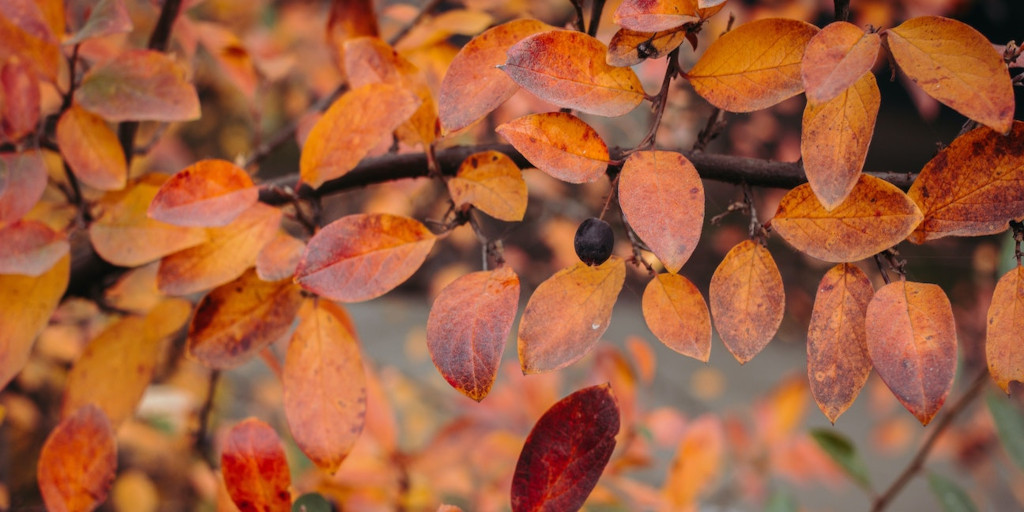
\includegraphics[scale=1]{images/orange2.jpg}
\caption{Maecenas varius orci vitae eros euismod placerat} \label{fig:integer}
\end{figure}

\subsection{Convallis quis elementum feugiat}

Rutrum in ligula. Nulla ut semper ligula, sed lobortis enim. Vivamus nulla eros,
faucibus ac convallis in, ornare at elit. Aliquam erat odio, finibus at purus ut,
porta ullamcorper odio. Vivamus ac augue tincidunt, semper magna volutpat,
condimentum sem. Praesent eget neque vitae odio volutpat vulputate.


% =======================================================================================
%                                   PART II
% =======================================================================================
% \part{Dolor sit amet}
%----------------------------------------------------------------------------------------
\newpage
\chapter{Hendrerit sapien} \label{ch:hendrerit}
\section{Sed ultrices} \label{sec:sed-ultrices}

\subsection{Donec pellentesque}

Tempus ipsum, vitae condimentum nisi efficitur id. In velit mauris, auctor eget
sapien nec, viverra mattis neque. Nunc vel commodo nunc, eget cursus ex.

\begin{enumerate}
\item{Nunc maximus consequat tristique.}
\item{Praesent luctus ex aliquam rhoncus consectetur.}
\item{Suspendisse mattis velit ante, vitae mollis est pharetra a.}
\item{Duis tincidunt, urna id auctor imperdiet, odio dui ullamcorper nisi.}
\item{Integer tincidunt enim vitae nulla iaculis, in varius metus blandit.}
\item{Nunc quam arcu, fermentum non dapibus condimentum, condimentum eget nunc.}
\end{enumerate}

\subsection{Euismod sodales}

\begin{outline}
\lipsum[2]
\end{outline}

\subsection{Pellentesque a nulla}

\begin{lstlisting}[language=Solidity]
contract KingOfTheHill is Ownable {
    address public owner; // different from the owner in Ownable

    function () public payable {
        if(msg.value > jackpot) owner = msg.sender; // local owner
        jackpot += msg.value;
    }
    function takeAll () public onlyOwner { // contract creator
        msg.sender.transfer(this.balance);
        jackpot = 0;
    }
}
\end{lstlisting}

\newpage
\section{Phasellus tristique} \label{sec:phasellus-tristique}

Lacus ac turpis semper fringilla. Mauris fermentum varius neque, vel congue
elit tempus quis. Aliquam a nunc in nunc consectetur hendrerit ut quis felis. 

Quisque id dui magna. Curabitur posuere nisl at magna vehicula aliquam \ref{fig:duis}.
Duis et suscipit felis. Mauris non justo quis diam gravida placerat condimentum
ut sapien. Praesent imperdiet libero id est tincidunt ullamcorper.

\begin{figure}[ht]
\hspace*{-1.6cm}
\begin{tikzpicture}

\node (logs) [io] {Logs};
\node (storage) [io, right=2cm of logs] {Storage};
\node (log-topics) [io, below=1cm of logs] {Log: topics, data};

\node (parse-data) [block, below=1cm of log-topics] {Parse event arguments};
\node (arguments) [io, below=2.7cm of parse-data] {Event arguments};

\node (parse-selector) [block, left=2cm of parse-data] {Parse event selector};
\node (reverse-selector) [block, below=1cm of parse-selector] {Reverse selector};
\node (signature) [io, below=1cm of reverse-selector] {Event signature};

\node (identify-standard) [block, below=1cm of signature] {Identify standard and event};
\node (fetch-constraints) [block, below=1cm of identify-standard] {Fetch matching constraints};
\node (check-constraints) [decision, below=4.3cm of arguments] {Constraints?};

\node (references) [io, left=1.6cm of identify-standard] {References};
\node (rules) [io, left=2cm of fetch-constraints] {Rules};

\node (negative) [io, below=2cm of check-constraints] {False};
\node (positive) [io, right=2cm of negative] {True};

\node (c1) [container, fit=(parse-selector) (reverse-selector) (parse-data), draw=gray] {};

\node (c2) [container, fit=(identify-standard) (fetch-constraints), draw=gray] {};

\node (c3) [container, fit=(positive) (negative)] {};

\node (c4) [container, fit=(references) (rules)] {};

\node (c0) [container, fit=(log-topics) (c1) (c2) (check-constraints), inner ysep=6mm, yshift=-2mm] {};
\node (t0) [label, above=2mm of c0, xshift=-4cm] {Event poisoning?};

\draw [arrow] (logs) -- (log-topics);
\draw [arrow] (log-topics) -| (parse-selector);
\draw [arrow] (log-topics) -- (parse-data);
\draw [arrow] (parse-selector) -- (reverse-selector);
\draw [arrow] (reverse-selector) -- (signature);
\draw [arrow] (signature) -- (identify-standard);
\draw [arrow] (parse-data) -- (arguments);
% \draw [arrow] (arguments) |- (identify-standard);
\draw [arrow] (arguments) -- (check-constraints);
\draw [arrow] (identify-standard) -- (fetch-constraints);
\draw [arrow] (fetch-constraints) |- (check-constraints);
\draw [arrow] (references) -- (identify-standard);
\draw [arrow] (rules) -- (fetch-constraints);
\draw [arrow] (storage) -- +(0,-9cm) -| (check-constraints);
\draw [arrow] (check-constraints) -| node[label, near start, above] {no} (positive);
\draw [arrow] (check-constraints) -- node[label, near start, right] {yes} (negative);

\draw [arrow] (logs) edge [loop above] node[label, above] {Iterate} ();

\end{tikzpicture}
\caption{Maecenas hendrerit congue faucibus} \label{fig:duis}
\end{figure}


% =======================================================================================
%                                   APPENDICES
% =======================================================================================
% \part{Appendices}
%----------------------------------------------------------------------------------------
% \newpage
% \chapter{Vestibulum commodo} \label{ch:commodo}
% \section*{Integer semper dictum tellus}

Neque eu cursus faucibus, ipsum magna tincidunt dui, vel scelerisque urna nibh ut nisl:

\begin{description}[labelwidth=\widthof{\bfseries morbi convallis},align=left]
\item[Duis]{sit amet mattis magna.}
\item[Curabitur]{sit amet fermentum mi.}
\item[Morbi convallis]{purus eu fermentum accumsan, mauris felis consequat ipsum.}
\item[Ut]{sollicitudin sit amet tellus et mollis.}
\end{description}

\section*{A porttitor orci faucibus sit amet}

Vivamus et sapien vitae lacus ornare suscipit vitae id mauris:

\begin{description}[labelwidth=\widthof{\bfseries suspendisse},align=left]
\item[Vivamus]{in dui arcu.}
\item[Morbi]{vitae dolor libero.}
\item[Tellus]{est, pellentesque at ultrices non, consectetur sit amet augue.}
\item[Suspendisse]{elementum mollis nisl at aliquam.}
\end{description}

%----------------------------------------------------------------------------------------
% \newpage
% \chapter{Etiam facilisis} \label{ch:etiam}
% \section{Ipsum primis}

In faucibus orci luctus et ultrices posuere cubilia curae; Aliquam nunc ipsum,
sollicitudin ut tempus consectetur, fermentum at lectus.

Nullam molestie viverra \ref{sec:vestibulum} augue sit amet gravida.

\newenvironment{nomenclature}[1]
{
\begin{table}[hbt]
\caption{#1}
\begin{center}
\begin{tabular}{|l|l|l|}
\hline
\textbf{Symbol} & \textbf{Unit} & \textbf{Description}\\
\hline
}
{
\\\hline
\end{tabular}
\end{center}
\end{table}
}

\subsection{Mauris pellentesque}

\begin{nomenclature}{Massa sagittis malesuada}
$g$     & $m/s^{2}$ & nisi in mollis gravida
\end{nomenclature}

\subsection{Nulla massa}

\begin{nomenclature}{Quis imperdiet}
$Q_{p}$         & $t/h$             & consectetur tortor
\end{nomenclature}

\begin{nomenclature}{Magna lectus}
$\tau_{a}$    	& $^{\circ}C$       & integer mollis bibendum gravida\\
$f_{s}$     	& $/jour$           & vestibulum porta urna at ex dignissim tincidunt
\end{nomenclature}

\subsection{Nam vitae}

\begin{nomenclature}{Nibh a lacus tincidunt efficitur}
$X_n$   & $m$               & venenatis nisi\\
$Y_n$   & $m$               & integer malesuada eu ligula nec pharetra\\
$Z_n$   & $m$               & fusce non elit lectus
\end{nomenclature}

%----------------------------------------------------------------------------------------
\newpage
\listoffigures
\listoftables
%----------------------------------------------------------------------------------------
\newpage
\printbibliography[title = {Aliquam}]

\end{document}
